\graphicspath{{/Users/brunomedina/Dropbox/Tesis-Egobets/egobets-notas/resources/marco/}}
\chapter{Panorama general de las apuestas}


En este capítulo, se explora el panorama general de las apuestas para auxiliar al lector en la comprensión de la relevancia de Egobets en la industria de las apuestas y en el ámbito científico; también, se revisan las teorías relacionadas más destacadas y los estudios previos más sobresalientes. Finalmente, se dan a conocer las ligas que se estarán analizando y los motivos por las que fueron elegidas.

 \section{La fascinación por los juegos de azar}

Nadie conoce el origen de las apuestas, algunos dicen que todo comenzó con un anónimo paleolítico que rodó unos cuantos huesos para decidir hacia que dirección ir a cazar \cite{schwartz2013roll}. Más adelante, tanto los antiguos griegos como los etruscos examinarían la forma y las características del higado de una oveja para tomar las mejores decisiones para su futuro\footnote{Los adivinos llamados ``Arúspices'' eran los encargados de llevar la tarea de precedir el futuro en función de la examinación de las entrañas de varias bestias.}. Siglos después, los romanos usarían los huesos astrágalos (Ver figura~\ref{Fig:huesos}) de animales como precursores a los dados \cite{schwartz2013roll}.

\begin{figure}[!htb]\centering
   \begin {minipage}{0.85\textwidth}
     \frame{\includegraphics[width=\linewidth]{huesos}}
     \caption{Astrágalos, los predecesores de los dados}\label{Fig:huesos}
   \end{minipage}
\end{figure}

Hoy en día, las apuestas representan uno de los negocios más redituables del mundo. En 2013, se estimó que las ganancias brutas de esta industria sumaron más de cuatroscientos cuarenta mil millones de dólares\footnote{Acorde a la empresa de Inteligencia de Mercado ``H2 Gambling Capital'' \cite{economistHouseWins}.}. Como se puede observar en la figura~\ref{Fig:gasto-apuestas}, Estados Unidos encabeza la lista como el país que más gasta en apuestas, seguido por China. También se advierte que los residentes de Australia y Singapur apuestan mucho más agresivamente que los de cualquier otro país. Para terminar, en esta misma gráfica se estima que para el 2018 el gasto en apuestas será de más de quinientos mil millones de dólares.


\begin{figure}[!htb]\centering
   \begin {minipage}{0.85\textwidth}
     \frame{\includegraphics[width=\linewidth]{apuestas}}
     \caption{Miles de millones de dólares en apuestas}\label{Fig:gasto-apuestas}
   \end{minipage}
\end{figure}

Con estos datos, la relevancia de la industria de las apuestas en el mundo se vuelve evidente.  Por otra parte, con respecto a las apuestas en línea, la firma KPMG \cite{kpmgOnlineGaming} reporta que el mercado global de apuestas en línea creció un cuarenta y dos por ciento de Veintún mil doscientos millones de dólares en 2008 a Treinta mil millones de dólares en 2012. Este porcentaje es notablemente superior al quince por ciento esperado para el crecimiento del total de la industria de apuestas para el mismo periodo. 

Específicamente en Estados Unidos, Goldman Sachs valoró en 2009 que el mercado de apuestas en línea en caso de ser legalizado\footnote{El ``Unlawful Internet Gambling Enforcement Act of 2006'' (UIGEA)  prohíbe a los bancos y a las compañías de tarjetas de credito procesar cargos relacionados a casinos en línea. Según Alexander, G. \cite{alexander2008us} las cuatro preocupaciones federales principales detrás de este acto son: Primero, el internet provee un acceso fácil a las apuestas, esto podría exacerbar las tentaciones que enfrentan los apostadores compulsivos. Segundo, es muy complicado verificar la mayoría de edad a través de un sitio de apuestas. Tercero, los casinos en linea tienen un incentivo para defraudar a los usuarios gracias a la falta de regulación de la industria. Y cuarto, dado el volumen, la velocidad, el alcance internacional de la transacciones realizadas en internet y el alto nivel de anonimidad que tienen los operadores de casinos electrónicos; los oficiales federales creen que las apuestas en línea son particularmente suceptibles al lavado de dinero.} podría valer hasta doce mil millones de dólares \cite{goldmanParty}.En este mismo documento de KPMG \cite{kpmgOnlineGaming}, México se propone como un mercado potencialmente lucrativo. Una de las principales razones es la legislación que permite el juego en línea\footnote{En 2004, la Ley Federal de Juegos con Apuestas y Sorteos permitió y reguló los Juegos en Línea.}. La otra razón, el valor del mercado mexicano del juego en línea se estima en cuatro mil seiscientos millones de dólares \cite{yogonet}.

 \section{La casa siempre gana}



%Que no les gustó mi "INSPIRATIONAL QUOTE"
\begin{chapquote}{Adam Smith, \textit{Filósofo} \cite{smith1963wealth}}
	``No hay proposición más cierta en matemáticas que la siguiente: Entre más boletos [de lotería] compre, más probabilidades tiene de ser un perdedor. Compre todos los boletos de la lotería y pierda con certeza; cuanto más boletos compre, más cerca estará de esta certeza''
\end{chapquote}

%A ver así:
% \begin{savequote}[0.55\linewidth]
% ``No hay proposición más cierta en matemáticas que la siguiente: Entre más boletos [de lotería] compre, más probabilidades tiene de ser un perdedor. Compre todos los boletos de la lotería y pierda con certeza; cuanto más boletos compre, más cerca estará de esta certeza''
% \qauthor{Adam Smith, \textit{Filósofo} \cite{smith1963wealth}}
% \end{savequote}
% ok....  no jaló...


El principio básico detrás de un casino es muy sencillo: \emph{la ventaja de la casa}. Cada uno de los juegos que ofrece el casino tiene detrás un robusto sustento matemático, de manera que a pesar de aparentar ser un juego justo, le confiere a la casa una ventaja porcentual sobre el conjunto de jugadores. Al final del día, esta ventaja y la ley de los grandes números, le garantizan a los casinos que a largo plazo tendrán suficientes ganancias para subsistir, mantener su operación y gozar de utilidades sorprendentes. Sin embargo, no hay que olvidar que los fenomenos estudiados siguen siendo producto del azar, por lo que una buena racha de algunos ``Grandes Apostadores'' podría llegar a asustar aun a los dueños  más racionales de casinos \cite{hannum2005practical}.



Según Hannum \cite{hannum2005practical} hay dos grandes razones por las que la gente apuesta:

\begin{enumerate}
	\item \textbf{Entretenimiento.} Un individuo podría utilizar mil pesos para ir a un casino o a un concierto. Si la ventaja de la casa es muy grande y la persona pierde su dinero rápidamente, entonces la experiencia del entreteniminto del casino no sería apreciada por el jugador. Por el otro lado, si el casino logra entretener a la persona por una tarde mientras le regala bebidas y comida, entonces puede que este individuo repita la experiencia y nunca más asista a un concierto.
	\item \textbf{Cambio de Vida.} Si una persona ahorrara cien pesos semanalmente, al final del un año tendría cinco mil doscientos pesos. Pero si ese dinero lo gastara para comprar boletos de lotería, tendría la posibilidad de ganarse cuarenta millones de pesos. Claramente la probabilidad es muy cercana a cero; sin embargo, este gasto podría ser visto por esta persona como una única oportunidad para cambiar su vida.

\end{enumerate}

\emph{La ventaja de la casa}, se puede entender mejor analizando cada uno de los juegos que ofrece el casino y las probabilidades de ganar que tienen los jugadores. Tómese por ejemplo el juego de la ruleta americana\footnote{El juego de la ruleta americana consiste en 38 casillas que alternan 18 casillas rojas, 18 casillas negras y 2 casillas verdes. Cuando el crupier hace girar la ruleta, de manera aleatoria cae una pelotita en una de las casillas. Los jugadores apuestan sobre la posición final de la pelotita.}:
Cuando un jugador apuesta sobre el color negro (i.e. que la pelotita caiga sobre alguna de las casillas negras) entonces se tiene que la probabilidad de que el jugador gane la apuesta es de:\\
\[p\{\text{La pelotita caiga en casilla negra}\} = \frac{\text{\# casillas negras}}{ \text{\# casillas totales}}  = \frac{18}{38}\]\\

Afortunadamente para la casa, hay $2$ casillas que no son color negro ni rojo, por lo que de las $38$ casillas sólo $36$  tienen estos colores. Por lo tanto, la probabilidaad de que la pelotita caiga en una casilla verde es la siguente:

\[p\{\text{La pelotita no caiga ni en casillas rojas ni en negras}\} =\] 
\[\frac{\text{\# casillas totales - (\# casillas rojas + \# casillas negras)}}{ \text{\# casillas totales}}  =\]
\[\frac{38-18-18}{38} = \frac{2}{38}  \]

Estos $\frac{2}{38}$ son la ventaja de la casa, ya que cuando un jugador apuesta al color negro en la ruleta y acierta, recibe la misma cantidad de dinero que podría perder. Sin embargo, apostó a ganar con una probabilidad de $\frac{18}{38}$, pero la probabilidad de perder la apuesta es igual a $1 - \frac{18}{38} = \frac{20}{38}$. Este detalle hace importante ver el valor esperado que tiene esta apuesta para el jugador:
\[E[\text{Apostar }k\text{ pesos al color negro}] = k  \cdot   p\{\text{La pelotita caiga en casilla negras}\} \]
\[- k  \cdot   p\{\text{La pelotita no caiga en casilla negra}\} = k \cdot \frac{18-20}{38}= - k \cdot \frac{2}{38}\]

Dado que siempre que se apuesta $k>0$, esto implica que:
\[E[\text{Apostar }k\text{ pesos al color negro}] = - k \cdot \frac{2}{38} < 0; \forall k \in \mathbb{N} \]
Este resultado quiere decir que a la larga el jugador \textbf{siempre} va a terminar perdiendo dinero.
En un principio, $\frac{2}{38}$ de probabilidad pareciera poco, pero al multiplicarlo por la gran cantidad de jugadores y apuestas que se realizan en los casinos el monto final se vuelve exorbitante.

Este sencillo ejercicio ejemplifica como todos los juegos que se tienen en los casinos ofrecen una ventaja para la casa. Es interesante mencionar, que además de los juegos de azar como la ruleta, hay juegos que obligan al jugador a tener cierta habilidad para no perder su dinero tan rápidamente, este es el caso de juegos como el Blackjack que le dan a la casa ventajas más pequeñas al enfrentarse a jugadores expertos. La ventaja de la casa sustenta las ganancias del casino, sin embargo calcular esta ventaja puede llegar a ser  complicado y requerir un análisis matemático mucho más sofisticado e incluso se puede llegar a necesitar programar el juego para correr simulaciones y estimar estas probabilidades.

\begin{table}[ht]
\centering
\resizebox{\textwidth}{!}{%
\begin{tabular}{|l|c|}
\hline
\textbf{Juego}                            & \textbf{Ventaja de la Casa} \\ \hline
Ruleta (con doble cero)                   & 5.3\%                       \\ \hline
Dados (pass/come)                         & 1.4\%                       \\ \hline
Dados (pass/come con momios dobles)       & 0.6\%                       \\ \hline
Blackjack - jugador promedio              & 2.0\%                       \\ \hline
Blackjack - 6 barajas, estrategia básica  & 0.5\%                       \\ \hline
Blackjack - una baraja, estrategia básica & 0.0\%                       \\ \hline
Baccarat (sin apuestas de empate)         & 1.2\%                       \\ \hline
Caribbean Stud                            & 5.2\%                       \\ \hline
Let It Ride                               & 3.5\%                       \\ \hline
Poker de tres cartas                      & 3.4\%                       \\ \hline
Pai Gow Poker (ante/play)                 & 2.5\%                       \\ \hline
Tragamonedas                              & 5\% - 10\%                  \\ \hline
Video Poker                               & 0.5\% - 3\%                 \\ \hline
Keno (promedio)                           & 27.0\%                      \\ \hline
\end{tabular}
}
\caption{Ventajas de la casa para juegos populares de casino \cite{hannum2005practical}}
\label{ventaja-casa}
\end{table}

Finalmente, aun sin la ventaja de la casa se deber recordar que existe un famoso problema y su corolario que garantizan que la casa siempre gane: \emph{La ruina del Jugador} \cite[p.~95-99]{ross2006first}. Este problema enfrentado por varios famosos matemáticos\footnote{Se dice que Blaise Pascal se lo planteó a Pierre Fermat en 1656 \cite{edwards1983pascal}. Después Fermat se lo replanteo a Christian Huygens en 1657 y finalmente James Bernoulli lo resolvió en su forma general como el problema de la ``Duración de Juego''. Fue publicado ocho años después de la muerte de Bernoulli en 1713 \cite[p.~98]{ross2006first}.} deja la siguiente lección: La probabilidad de que un jugador pierda todo su dinero es igual a  $p_1 = \frac{n_2}{n_1 + n_2}$ donde $p_1$ es la probabildad de ganar del jugador $1$ y $n_i$ es la cantidad de dinero que va a apostar el jugador $i$. Desafortunadamente, usualmente la casa tendrá más dinero para apostar que cualquier jugador, por lo que con esta fórmula la casa siempre gana\footnote{Ver demostración en el apéndice~\ref{chap:ruina}.}.


 \section{Mercados de apuestas deportivas}
 
 A diferencia de las máquinas tragamonedas y los juegos de mesa de los casinos, las apuestas deportivas tienen una gran ventaja para los apostadores: los resultados de los encuentros deportivos \textbf{no son completamente aleatorios,} ya que dependen en cierta medida del nivel de juego que tienen los equipos participantes. Hannum menciona en su libro \cite{hannum2005practical} : \emph{``La ventaja de la casa existe para casi todas las apuestas en un casino (ignorando las salas de Poker y las apuestas deportivas donde algunos pocos profesionales pueden vivir de de las apuestas)''}

 Existen dos grandes mercados en esta rama de las apuestas \cite{chung2010empirical}:
 \begin{itemize} 
 	\item \emph{Bookies.}\footnote{``Bookie'' proviene de la palabra en inglés ``bookmakers'' que en español se utiliza como: ``Corredor de apuestas''.} El corredor de apuestas analiza los diferentes resultados de un encuentro deportivo en función de los participantes. Con base en este análisis, el bookie publica un número (llamado \emph{``momio''}) para cada uno de los posibles desenlaces del partido. Este ``momio'' representa la cantidad potencial de retorno de esa apuesta (incluída la cantidad de dinero arriesgada)\footnote{Por ejemplo, supongase que se apuestan cien dólares a favor del empate de un partido con un momio igual a $3.640$. En caso de que se ganara la apuesta, el jugador recibíria la cantidad de $(100)(3.640) = 364$ dólares. Sustrayendo los cien dólares que apostó, su ganancia neta sería de $264$ dólares.}. El bookie recibe apuestas sobre estos momios y cobra una comisión por cada operación recibida. 
 	\item \emph{Sistema parimutual.} En este mercado no existen  corredores, ni momios. El pago que reciben los jugadores depende de la cantidad de dinero recopilada por todas las apuestas recibidas. Por lo tanto, las ganancias de los jugadores no están determinadas hasta que todas las apuestas se reciben\footnote{Las afamadas ``quinielas'' son un tipo de apuesta de mercado parimutual.}.
 	\end{itemize}

 Aunque la eficiencia\footnote{Fama, E \cite{fama1998market} sugiere que la eficiencia de mercado es cuando los precios reflejan completamente toda la información disponible de una acción en particular.} de estos mercados no es un tema que se aborde a profundidad en esta tesis, es interesante mencionar que ha sido  muy cuestionada. Sauer \cite{sauer1998economics} y Williams \cite{williams1999information} critican varias de sus anomalías; por ejemplo hay un problema interesante en la eficiencia del mercado de las apuestas de los bookies conocido como: Sesgo del \emph{``favorite - long shot''.} Estos autores explican que las apuestas a los equipos favoritos generan un mayor retorno de dinero en comparación con el retorno generado por las apuestas a equipos cuyas probabilidades de ganar son mucho menores (``longshot bets''). Incluso se han realizado varios estudios proponiendo un nuevo mercado de tipo ``doble subasta'' que consiste en tener compradores y vendedores proponiendo los precios de la apuesta, cuando dos de ellos coinciden, se lleva acabo la transacción. Referirse a Ozgit\cite{ozgit2005posted}.

 El mercado pertinente para este trabajo es el de los ``bookies'' o corredores de apuestas. Sin embargo, bajo las condiciones adecuadas la asesoría de apuestas podría ayudar a los jugadores en el mercado parimutual. Por ejemplo, en una apuesta entre compañeros del trabajo el usuario del sistema podría indagar la apuesta realizada por cada uno de los participantes y conocer la cantidad de retorno que tiene de cada uno de los resultados. Si el sistema de Egobets le recomendara realizar esta apuesta en particular, bastaría verificar que el retorno del pago sea mejor que el pago que realizan las casas de apuestas en general. Realizando esta acción sistemáticamente, se podrían conseguir mejores ganancias que las ofrecidas por el mercado.

 Sin importar el mercado, es importante tomar en cuenta el hecho de que las probabilidades reales que tienen los distintos resultados de cualquier partido \textbf{son desconocidas}. Por lo que los ``bookies'' contratan a empresas consultoras, o designan un área de la compañía para calcular los momios que se publican en el mercado. Este punto es básico en la creación de sistemas como Egobets, ya que el hecho de que las probabilidades sean desconocidas permite que Egobets busque estimar probabilidades mucho más cercanas a las reales. Al minimizar el error de estimación que tienen las probabilidades sugeridas por las casas de apuestas, se pueden encontrar apuestas cuyo retorno sería mayor al que realmente debería ser. Y como se verá en la siguiente sección, este error de estimación siempre existirá, debido a que los momios publicados por las casas de apuestas no buscan reflejar las probabilidades reales de los resultados de los partidos.

 Una ventaja con la que cuentan los apostadores de eventos deportivos: si los bookies establecen mal sus momios\footnote{La cantidad de dinero que pagan las apuestas a eventos completamente aleatorios, como los juegos dentro de los casinos, se puede calcular explícitamente. Por lo que la única manera de que una de estas apuestas tuviera valor esperado positivo sería si se cometieron errores en los cálculos.}, entonces ciertos jugadores pueden llegar a tener valores esperados positivos en sus apuestas y con esto la casa podría llegar a perder mucho dinero, incluso a largo plazo (como se verá en la siguiente sección). Procédase a la siguiente sección para conocer los orígenes de los momios y las condiciones que permiten a los bookies ganar dinero con ellos.
 
 \section{Bookies y momios}
Ya que el objeto de estudio central de esta tesis toma lugar en el deporte del futbol, analícese la pregunta más recurrente de un partido de futbol: \emph{¿Qué equipo va a ganar este partido?}

La respuesta tiene $3$ posibilidades:
 \begin{enumerate}
  \item El partido lo gana el equipo de casa.
  \item Es un empate.
  \item El partido lo gana el equipo visitante.
 \end{enumerate}
 
En un principio se pudiera pensar que los tres eventos son equiprobables, pero como se mencionó en la sección anterior esto resulta imposible por muchísimas razones, como por ejemplo: ser el equipo visitante conlleva una desventaja importante en el desempeño del partido (Ver \cite{roffe2007crisis}), o la desventaja de tener a los jugadores estrella lesionados; incluso las condiciones climáticas (altitud, tipo de pasto, lluvia) durante el partido pueden ser determinantes para el resultado final. En un caso extremo, imagínese el escenario donde ambos equipos fueran igual de buenos en todos los aspectos. En este escenario, la probabilidad de empate sería mayor que las otras dos. Sin embargo, estas razones no son (tampoco) suficientes para calcular los resultados de los partidos de manera determinística. Gracias a estas particularidades es que el estudio de este mercado de apuestas se vuelve tan interesante.

Anteriormente se definió un momio como el número que indica la cantidad de dinero que obtiene un jugador al ganar una apuesta. Sin embargo, para generar los momios, las casas de apuesta realizan estudios minuciosos de mercado y de los deportes en sí mismos. Las probabilidades de cada resultado de un partido no son, de lejos, los únicos factores a considerar por el bookie a la hora de generar los momios.  

Levitt \cite{levitt2004gambling} menciona tres escenarios que permitirían a los bookies generar ganancias:
 \begin{enumerate}
  \item \textbf{Encontrar el precio de equilibrio.} Los bookies buscan predecir los momios\footnote{Antes del partido estos momios pueden llegar a tener ajustes tipicamente pequeños y relativamente infrecuentes.} que igualen el precio de equilibrio del mercado de apuestas. Es decir, se buscan los momios que equilibran la cantidad de dinero en cada lado de la apuesta. Esto implica que la diferencia de dinero entre todas las apuestas es igual a cero. Por lo que sin importar quien gane el partido, el bookie cobrará su comisión de las apuestas intacta y no tendrá deudas en ninguna de las apuestas.
  
  \item \textbf{Predecir los resultados del partido.} Si el bookie fuera sistemáticamente mejor en predecir los resultados de los partidos, entonces podría publicar el momio ``correcto'' del partido (i.e. el momio que equilibra la probabilidad de que una apuesta en cualquiera de los resultados gane). Aunque la cantidad de dinero no estaría equilibrada, en promedio el bookie ganaría la comisión cobrada a los jugadores. Nótese que a diferencia del primer escenario, en este esquema existe un riesgo enorme al que se exponen las casas de apuestas. Si llegaran a fijar un momio muy alejado del precio de equilibro del mercado, entonces podría darse el caso de que la cantidad de dinero a pagar a los ganadores de la apuesta sea mayor a la cantidad de dinero recaudada por las apuestas complementarias, lo que podría significar pérdidas millonarias para el bookie\footnote{Levitt \cite{levitt2004gambling} cuenta el ejemplo del Epson Derby de 1946, donde los momios fueron errados y la mitad de todas las casas de apuestas británicas se fueron a bancarrota.}.

 Ahora, tómese de ejemplo el siguiente partido con los siguientes momios:
 \begin{itemize}

 \item \textbf{Cagliari Vs Juventus.}
  \begin{itemize}
    \item \textbf{9.290} Gana local (Cagliari)
    \item \textbf{1.423} Empate.
    \item \textbf{4.760} Gana visitante (Juventus)
  \end{itemize}
 \end{itemize}

  Sea $m_i$ el momio que propone el bookie para que los jugadores apuesten a que se cumpla el evento $i$. Entonces, se define el momio de la siguiente manera:
 \[m_i = \frac{1}{1 - \hat{p_i}}\]
 Donde $\hat{p_i}$ es la probabilidad estimada que tiene el bookie de que suceda el evento $i$\footnote{Otros deportes tienen diferentes tipos de momios y su definición varía dependiendo del tipo de apuesta, se puede leer más de ellos en \cite{ignatin1984sports}.}

 Con estos momios se pueden calcular las ``probabilidades estimadas por el bookie'':
 \[\hat{p_L} = 1 - \frac{1}{9.290} \approx 0.107643...\] 
 \[\hat{p_E} = 1 - \frac{1}{1.423} \approx 0.702741...\]
 \[\hat{p_V} = 1 - \frac{1}{4.760} \approx 0.210084...\]
 Donde $\hat{p_L}$ es la probabilidad estimada por la casa de apuestas de que gane el equipo local, $\hat{p_E}$ es la probabilidad de que el partido termine en empate y $\hat{p_V}$ es la probabilidad de que gane el equipo visitante.
 
 Estas probabilidades estimadas proponen que el escenario más probable es un empate, después la victoria del Juventus y finalmente la victoria del Cagliari. Curiosamente en este ejemplo, se puede ver que aunque el equipo Cagliari es local, se enfrenta a un adversario que puede contra la desventaja de ser visitante.

 Uno de los teoremas básicos de la probabilidad, dice que la suma de las probabilidades de todos los resultados del evento debe sumar uno \cite{ross2006first}. Sin embargo, en el caso de los bookies, las probabilidades estimadas exceden la unidad. Este excedente, es la vieja conocida: ``Ventaja de la Casa''.

 Sea $\mathcal{O}$ el conjunto de todas las opciones sobre las que un jugador puede apostar para cierto evento. Para el caso de las apuestas sobre los resultados de los partidos, se tiene que: $\mathcal{O} = \{\text{Apostar a que gane local}, \text{Apostar al empate}, \text{Apostar a que gane visitante}\}$.

 Por lo tanto:
 \[\text{Ventaja de la casa} =  \left(\sum_{i \in \mathcal{O}}{\left(1 - \frac{1}{\text{Momio de la opción } i}\right)}\right) - 1\] 

 Siguiendo con el ejemplo, se tiene que la ventaja de la casa de este bookie para esta apuesta en particular es:
 \[\text{Ventaja de la casa} = \hat{p_L} + \hat{p_E} + \hat{p_V} - 1 \approx 0.020467\]

 Este $2.046\%$ es el punto de partida que la casa quiere obtener en ganancias. 


  \item \textbf{Predecir los resultados y encontrar el precio de equilibrio.} Si el bookie es mejor que los jugadores prediciendo el resultado de los partidos y también puede encontar el precio de equilibrio, entonces podría con esta información mejorar sus ganacias esperadas al publicar un momio ``equivocado'' de tal manera que el momio (precio) de equilibrio quede posicionado donde sus ganancias se incrementen. Ahora, hay ciertas restricciones en cuanto a la distancia a la que puede quedar posicionado el momio ``equivocado'', ya que pueden existir jugadores que conozcan el momio ``correcto'' por lo que entre mayor sea esta distancia podría generar mayores ganancias para estos jugadores. Por ejemplo, supongase el siguiente caso extremo: Se disputa un partido entre los equipos $A$ y $B$, el equipo $B$ es el favorito para ganar. Es por esto que la casa de apuestas arregló que el partido lo gane el equipo $A$. El bookie conoce que la probabilidad de que el equipo $A$ gane el partido es $1$, es por esto que fija los momios más competitivos del mercado a favor del equipo $B$ y a favor del empate, mientras que el momio a favor del equipo $A$ lo presenta mucho menos competitivo que el resto del mercado. Con estas acciones, la casa de apuestas maximiza las apuestas recibidas en contra del equipo $A$ y minimiza las apuestas a favor del equipo $A$ dado que las otras casas de apuestas pagan mucho mejor este resultado. Ahora, si los momios fueran absurdamente buenos en contra del equipo $A$ ciertos apostadores podrían intuir que la casa de apuestas sabe algo que los demás no saben y podrían apostar cantidades exorbitantes a favor del equipo $A$.

  % Para el ejemplo anterior, si la casa conociera las probabilidades reales de los resultados del partido, entonces podría (por ejemplo) presentar para ese partido al equipo visitante (Juventus) como la mejor opción para la apuesta, cuando en realidad no lo es. Este tipo de técnicas aplicadas sistematicamente pueden ayudar al bookie a obtener ingresos mayores a largo plazo.
 \end{enumerate}


 De estos tres escenarios, Levitt \cite{levitt2004gambling} examina de un bookie en línea, veinte mil apuestas de doscientos ochenta y cinco jugadores para los partidos de la NFL\footnote{La liga de futbol americano más popular: National Football League.}. Esto fue lo que encontró:
 \begin{itemize}
  \item A pesar de ser un estudio para una sola casa de apuestas, sugiere que se pueden generalizar ya que casi todas las casas ofrecieron casi los mismos momios para los mismos partidos
  \item El bookie no parece buscar el precio de equilibrio del mercado. Acorde a los resultados en casi la mitad de todos los juegos al menos dos tercios de las operaciones caen en un solo lado de la apuesta.
  \item El bookie parece colocar precios estratégicamente para explotar los sesgos de los apostadores. Es decir, los jugadores parecen tener un sesgo sistemático hacia los equipos favoritos y, en menor medida, hacia los equipos visitantes. En consecuencia, el bookie logró atraer mayor atención a partidos donde estos equipos no tuvieron buenas actuaciones; estos precios lograron elevar las ganancias hasta un veinte por ciento más que con lo que hubieran obtenido en el primer escenario.
  \item Hay poca evidencia de que existan jugadores que hayan sido capaces de vencer a los bookies sistemáticamente.
  \end{itemize}
 
 Estas conclusiones indican que, al menos en el deporte del futbol americano, las casas de apuestas buscan siempre tener mayores ganancias. Es por esta razón que podrían estar usando el tercer escenario descrito previamente. Es interesante destacar que los momios, en realidad reflejan la probabilidad que el mercado cree que tiene cada resultado de un partido. Es por esto que sistemas como Egobets, que funcionan al aprovecharse de los momios ``equivocados'' propuestos por las casas de apuestas, pudieran llegar a funcionar satisfactoriamente.
 
 
 \section{La apuesta ganadora}

 \begin{enumerate}[(a)]
  \item Sean $p_L$, $p_z$, $p_v$ las probabilidades de que gane local, empaten o gane visitante, respectivamente. Sean $\mu_L$, $\mu_z$ y $\mu_v$ los momios respectivos. El problema de decisión de apostar \$\,1 en esta situación es:\\
 
 % Set the overall layout of the tree
 \tikzstyle{level 1}=[level distance=3.5cm, sibling distance=2.5cm]
 \tikzstyle{level 2}=[level distance=3.5cm, sibling distance=2cm]
 \tikzstyle{level 3}=[level distance=3.5cm, sibling distance=2cm]


 \begin{figure}[ht]
 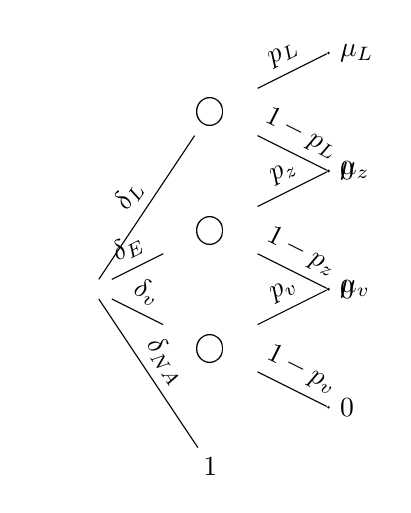
\begin{tikzpicture}[grow=right, sloped]
 \node[text width=4em, text centered] {$\square$}
 %%%%%%%%%%%%%%%%%%%%%%%%%%%%%%%%%%%%%%%%%%%%%%%%%
 %cuarto
 %%%%%%%%%%%%%%%%%%%%%%%%%%%%%%%%%%%%%%%%%%%%%%%%
 child {       
     node[text width=4em, text centered] {1}
              edge from parent         
  node[above] {$\delta_{NA}$}
     }
 %%%%%%%%%%%%%%%%%%%%%%%%%%%%%%%%%%%%%%%%%%%%%%%%%
 %tercero
 %%%%%%%%%%%%%%%%%%%%%%%%%%%%%%%%%%%%%%%%%%%%%%%%
 child {       
     node[text width=4em, text centered] {\textbigcircle}
     child {
                 node[circle, minimum width=1pt,fill, inner sep=0pt, label=right:
                     {$0$}] {}
                 edge from parent
                 node[above] {$1-p_v$}             
             }
             child {
                 node[circle, minimum width=1pt,fill, inner sep=0pt, label=right:
                     {$\mu_v$}] {}
                 edge from parent
                 node[above] {$p_v$}              
             }
              edge from parent         
  node[above] {$\delta_v$}
     }
 %%%%%%%%%%%%%%%%%%%%%%%%%%%%%%%%%%%%%%%%%%%%%%%
 %segundo
 %%%%%%%%%%%%%%%%%%%%%%%%%%%%%%%%%%%%%%%%%%%%%%%%
     child {       
     node[text width=4em, text centered] {\textbigcircle}
     child {
                 node[circle, minimum width=1pt,fill, inner sep=0pt, label=right:
                     {$0$}] {}
                 edge from parent
                 node[above] {$1-p_z$}             
             }
             child {
                 node[circle, minimum width=1pt,fill, inner sep=0pt, label=right:
                     {$\mu_z$}] {}
                 edge from parent
                 node[above] {$p_z$}              
             }
              edge from parent         
  node[above] {$\delta_E$}
     }
 %%%%%%%%%%%%%%%%%%%%%%%%%%%%%%%%%%%%%%%%%%%%%%%
 %primero
 %%%%%%%%%%%%%%%%%%%%%%%%%%%%%%%%%%%%%%%%%%%%%%%%
     child{
     node[text width=4em, text centered] {\textbigcircle}        
             child {
                 node[circle, minimum width=1pt,fill, inner sep=0pt, label=right:
                     {$0$}] {}
                 edge from parent
                 node[above] {$1-p_L$}             
             }
             child {
                 node[circle, minimum width=1pt,fill, inner sep=0pt, label=right:
                     {$\mu_L$}] {}
                 edge from parent
                 node[above] {$p_L$}              
             }    
  edge from parent         
  node[above] {$\delta_L$}
     };  
 \end{tikzpicture}
 \caption{Decidir por quién apostar}
 \end{figure}

   $E_p[U(\delta_i)]=p_i\mu_i;\quad i=L,Z,V$\\
  
   Sol: Se escoge $\rho_i \,\, \cdot \ni \cdot \,\, E_p[U(\delta_i)]=max\{p_L\mu_L,p_z\mu_z,p_v\mu_v,1\}$
  
   \item Se quiere decidir si apostar o no en la ocurrencia de un evento: Sea $p=p(E)$ y $f_p$ densidad de $p$. Sea $\mu$ el momio en el caso de ocurrencia. El problema de decisión asociado es el siguiente:\\
 
 \begin{figure}[!ht]
  \begin{tikzpicture}[grow=right, sloped]
 \node[text width=4em, text centered] {$\square$}
 %%%%%%%%%%%%%%%%%%%%%%%%%%%%%%%%%%%%%%%%%%%%%%%%%
 %segundo
 %%%%%%%%%%%%%%%%%%%%%%%%%%%%%%%%%%%%%%%%%%%%%%%%
 child {       
     node[text width=4em, text centered] {0}
              edge from parent         
  node[above] {$\delta_{NA}$}
     }
 %%%%%%%%%%%%%%%%%%%%%%%%%%%%%%%%%%%%%%%%%%%%%%%
 %primero
 %%%%%%%%%%%%%%%%%%%%%%%%%%%%%%%%%%%%%%%%%%%%%%%%
     child{
     node[text width=4em, text centered]{\textbigcircle}
    	    child {
    	        node[]{\textbigcircle}   	                 
                 %node[above] {$f_p$}
                 child{node[circle, minimum width=1pt,fill, inner sep=0pt, label=right:
                     {$-1$}] {}                    
                 edge from parent
                 node[above] {$1-p$}             
             }
             child {
                 node[circle, minimum width=1pt,fill, inner sep=0pt, label=right:
                     {$\mu-1$}] {}
                 edge from parent
                 node[above] {$p$}              
             }
             edge from parent
             node[above] {$f_p$}}    
  edge from parent         
  node[above] {$\delta_A$}
     };
 \end{tikzpicture}  
 \caption{Decidir si apostar o no apostar}
 \end{figure}
 
 \newpage
  
   $\rightarrow E_p[U(\delta_A)]=E_{f_p}[p(\mu-1)-(1-p)]\\
   =E_{f_p}[p(\mu)-1]\\
   =E_{f_p}(p)\mu-1$\\

   Apuestas si $E_{f_p}(P)\cdot \mu \ge 1$
  
   \item Mismo problema que el caso anterior, sólo que la utilidad depende de $p$ y $\mu$: $U: \Re\times[0,1]\rightarrow\Re$\\
   $(U(0,p)=0\quad\forall p)$.\\
 
 \begin{figure}[ht]
 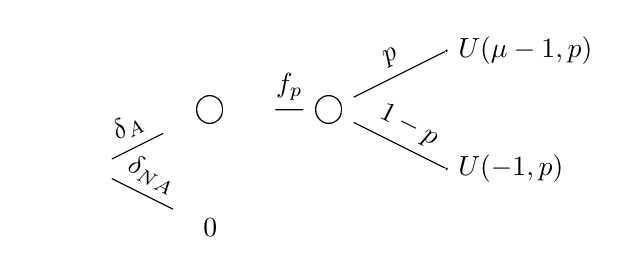
\begin{tikzpicture}[grow=right, sloped]
 \node[text width=4em, text centered] {$\square$}
 %%%%%%%%%%%%%%%%%%%%%%%%%%%%%%%%%%%%%%%%%%%%%%%%%
 %segundo
 %%%%%%%%%%%%%%%%%%%%%%%%%%%%%%%%%%%%%%%%%%%%%%%%
 child {       
     node[text width=4em, text centered] {0}
              edge from parent         
  node[above] {$\delta_{NA}$}
     }
 %%%%%%%%%%%%%%%%%%%%%%%%%%%%%%%%%%%%%%%%%%%%%%%
 %primero
 %%%%%%%%%%%%%%%%%%%%%%%%%%%%%%%%%%%%%%%%%%%%%%%%
     child{
     node[text width=4em, text centered]{\textbigcircle}
    	    child {
    	        node[]{\textbigcircle}   	                 
                 %node[above] {$f_p$}
                 child{node[circle, minimum width=1pt,fill, inner sep=0pt, label=right:
                     {$U(-1,p)$}] {}                    
                 edge from parent
                 node[above] {$1-p$}             
             }
             child {
                 node[circle, minimum width=1pt,fill, inner sep=0pt, label=right:
                     {$U(\mu-1,p)$}] {}
                 edge from parent
                 node[above] {$p$}              
             }
             edge from parent
             node[above] {$f_p$}}    
  edge from parent         
  node[above] {$\delta_A$}
     };
 \end{tikzpicture}
 \caption{Decidir si apostar en función de una utilidad}
 \end{figure}

  
  
   Se apuesta si: \\
   $E_p(U(\delta_A))=E_p[p\,U(\mu-1,p)+(1-p)U(-1,p)]\ge0$
 \end{enumerate}

 Algunas funciones de utilidad posibles:
 \begin{itemize}
  \item $U_\mu(x,p)=x(\frac{1}{\mu}-p)^2$\\
 
  Notese que: $p\,U_\mu(\mu-1,p)+(1-p)U_\mu(-1,p)$\\
 
  $(\hat p=\frac{1}{\mu})=(\hat p-p)^2(p\mu-1)$\\
 
  Me duele más mientras más alejado esté de un trato beneficioso y me produce mayor placer mientras mayor sea el beneficio del trato.
 
  \item $U_{\mu,a}(x,p)= \left\{ \begin{array}{lcc}
              ax(\hat p-p)^2 &   si  & p \le \hat p \\
              & &\\
              x (\hat p-p)^2 &  si & p>\hat p\\             
              \end{array}
  \right.$
 
  Notese que: \\
  \[U_\mu=U_{\mu,1}\]\\
  \[p\,U_{\mu,a}(\mu-1,p)+(1-p)U_\mu(-1,p)= \left\{ \begin{array}{lcc}
              a(\hat p-p)^2 (p\mu-1)&   si  & p \le \hat p \\
              & &\\
              (\hat p-p)^2(p\mu-1) &  si & p>\hat p\\             
              \end{array}
  \right.\]

  Me duele ``a'' veces más un trato perjudicial  que un trato beneficioso si me encuentro a la mis ma distancia que $\hat p$.
 
  \item $U_{\mu,a,b}=U_{\frac{\mu}{1+\mu b},a}$\\
 
  y considerar el problema de decisión con $\mu'=\frac{\mu}{1+\mu b}$.\\
 
  Si $\mu'=\frac{\mu}{1+\mu b}\rightarrow \hat p'=\hat p+b$.\\
 
  Los tratos empiezan a ser beneficiosos hasta que el menos sea $b\%$ más probable que ocurra el evento de lo que sería justo.\\
 
  {\bf Nota:} En un problema de decisión sin aversión a la distribución de probabilidades (o con probabilidades fijas) si se desea apostar en apuestas con un mínimo de ganancias esperadas igual a $b\%$ se debe comparar $\mu_p$ con $1+b$ (i.e. apostar $\leftrightarrow \mu_p \ge 1+b$).
 
 \end{itemize}

 \section{Decidir la cantidad de dinero a apostar}

 Supongamos que $\mu_p \ge 1$ y que existen 2 funciones de utilidad:
 \[U_1:\Re^+ \rightarrow \Re^+\]
 \[U_2:\Re^+ \rightarrow \Re^+\]

 La primera es la función de utilidad del dinero para las ganancias y la segunda es la utilidad del dinero para las pérdidas monetarias.\\

 Se harán las siguientes supuestos:

 \begin{enumerate}[(i)]
  \item $U_1(0)=U_2(0)=0$. $U_1$, $U_2$ no decrecientes, una vez cont. dif.
  \item $U'_1(0)>U'_2(0)$ (por lo tanto convendrá apostar).
  \item $\forall M>0$ fija $\displaystyle \lim_{x\rightarrow \infty} \frac{U_1(\mu x)}{U_2(x)}=0$.\\
  (Perder duele muchisimo más que ganar).
 \end{enumerate}
 El problema de decisión asociado a  determinar la cantidad óptima a postar es:(con $0<p<1$ fija y $\mu$ momio)\\

 \begin{figure}[ht]
  \begin{center}
 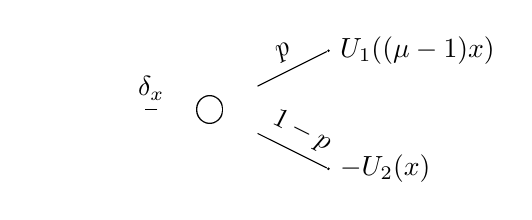
\begin{tikzpicture}[grow=right, sloped]
 \node[text width=4em, text centered] {$\square$}
 %%%%%%%%%%%%%%%%%%%%%%%%%%%%%%%%%%%%%%%%%%%%%%%
 %primero
 %%%%%%%%%%%%%%%%%%%%%%%%%%%%%%%%%%%%%%%%%%%%%%%%
 child{
     node[text width=4em, text centered] {\textbigcircle}        
             child {
                 node[circle, minimum width=1pt,fill, inner sep=0pt, label=right:
                     {$-U_2(x)$}] {}
                 edge from parent
                 node[above] {$1-p$}             
             }
             child {
                 node[circle, minimum width=1pt,fill, inner sep=0pt, label=right:
                     {$U_1((\mu-1)x)$}] {}
                 edge from parent
                 node[above] {$p$}              
             }    
  edge from parent         
  node[above] {$\delta_x$}
     };
 \end{tikzpicture} 
 \end{center}
 \caption{Árbol de probabilidad 4}
 \end{figure}



 $\rightarrow E_p[U(\delta x)]=pU_1((\mu-1)x)-(1-p)U_2(x)$\\

 Sea $f(x)=E_p[U(\delta x)]$\\

 Encontrar el óptimo es encontrar $x \ge 0$ que resuelva el problema: $\displaystyle \max_{x\ge0}f(x)$\\

 \[f'(x)=p(\mu-1)U'_1((\mu-1)x)-(1-p)U'_2(x)=0\]
 \[\frac{p(\mu-1)}{(1-p)}=\frac{U'_2(x)}{U'_1((\mu-1)x)}\]
 P.d.$$\exists \quad x^* \quad \cdot \ni \cdot \quad \frac{p(\mu-1)}{1-p}=\frac{U'_2(x)}{U'_1(\mu x)}$$

 \begin{enumerate}[(i)]

  \item $f'(0)=p(\mu-1)U'_1(0)-(1-p)U'_2(0)>p(\mu-1)U'_2(0)-(1-p)U'_2(0)$\\
 
  $\,\,\,\quad\quad=U'_2(0)(p\,\mu-1)\ge 0$\\
 
  Con $U_2'(0)\ge 0$ y $p\mu\ge0$\\
  Por tanto $f'(0)>0$
 
  \item $f(0)=0$
  \item $\displaystyle\frac{f(x)}{U_2(x)}=p\displaystyle\frac{U_1((\mu-1)x)}{U_2(x)}-(1-p)$\\
  $\rightarrow \displaystyle \lim_{x\rightarrow\infty}\frac{f(x)}{U_2(x)}=-(1-p)$\\
 
  $\rightarrow \exists \, x\,\,\cdot \ni \cdot \,\, \displaystyle\frac{f(x)}{U_2(x)}=-(1+p)+\varepsilon<0$\\
 
  $\rightarrow \exists\,x\,\,\cdot \ni \cdot \,\,f(x)<0$
  \begin{itemize}
   \item Por $T.V.M.\,\,\,\exists\,\, x'\in(0,x)\,\,\cdot \ni \cdot \,\,xf'(x')=f(x)-f(0)=f(x)<0$\\
   $\rightarrow f'(x')<0$
   \item T.V.I. $\exists\,\, x^*\in(0,x')\,\,\cdot \ni \cdot \,\,f'(x^*)=0$. i.e. $\displaystyle\frac{p(\mu-1)}{1-p}=\displaystyle\frac{U'_2(x)}{U'_1(\mu x)}$\\
  
   Como $f$ es primero creciente y en algún punto decreciente:\\
   $\rightarrow x\,\,\cdot \ni\cdot\,\,f'(x)=0$ es un maximizador.
  \end{itemize}
 \end{enumerate}

 Algunas funciones a considerar:
 \begin{itemize}
  \item $U_{1,\alpha}(x)=x^{\alpha}\qquad\qquad 0<\alpha<1$\\ 
  $U_2(x)=x$\\
 
  Compruébense los supuestos:
  \begin{enumerate}[(i)]
   \item $U_{1,\alpha}(0)=0=U_2(0)$, son crecientes y una vez dif.
   \item $U'_{1,\alpha}(0)=+\infty$, $U'_2(0)=1\qquad{\therefore \,\, U'_{1,\alpha}(0)>U'_2(0)}$
   \item $\forall \,\, \mu>0$\\
  
   $\displaystyle\lim_{x\rightarrow +\infty}\displaystyle\frac{U_{1,\alpha}(\mu x)}{U_2(x)}=\mu^{\alpha}\displaystyle\lim_{x\rightarrow +\infty}\displaystyle\frac{x^{\alpha}}{x}=\mu^{\alpha}\displaystyle\lim_{x\rightarrow +\infty}\displaystyle\frac{1}{x^{1-\alpha}}=0$\\
  
   Para una apuesta con probabilidad $p$ y momio $\mu$ el óptimo se da en:\\
  
   $\displaystyle{\frac{p(\mu-1)}{(1-p)}=\frac{U'_2(x)}{U'_{1,\alpha}((\mu-1)x)}=\frac{1}{\alpha((\mu-1)x)^{\alpha-1}}=\frac{1}{\alpha}(\mu-1)^{1-\alpha}x^{1-\alpha}}$\\\\
  
   $\rightarrow \left(\displaystyle\frac{\alpha p}{(1-p)}\right)(\mu-1)^{\alpha}=x^{1-\alpha}\rightarrow x^*=\left(\displaystyle\frac{\alpha p}{1-p}\right)^{\frac{1}{1-\alpha}}(\mu-1)^{\alpha/1-\alpha}$\\
  \end{enumerate}

  \item $U_{1,\alpha}(x)=x^{\alpha}\qquad\qquad 0<\alpha<1$\\
  $U_{2,\beta}(x)=x^{\beta}\qquad\qquad \beta \le1$\\
 
  Es fácil revisar los supuestos. Para una apuesta con probabilidad $p$ y momio $\mu$ el óptimo se da en:\\
 
  ${\displaystyle\frac{p(\mu-1)}{(1-p)}=\frac{\beta x^{\beta-1}}{\alpha(\mu-1)^{\alpha-1}x^{\alpha-1}}=\frac{\beta}{\alpha}(\mu-1)^{1-\alpha}x^{\beta-\alpha}}$\\
 
  $\rightarrow{\displaystyle\left(\frac{\alpha p}{\beta(1-p)}\right)(\mu-1)^{\alpha}=x^{\beta-\alpha}\rightarrow x^*=\left(\frac{\alpha p}{\beta(1-p)}\right)^{1/\beta-\alpha}(\mu-1)^{\alpha/\beta-\alpha}}$
 
  \item $U_1(x)=\ln (x)$\\
  $U_2(x)=x$\\
 
  Es fácil revisar los supuestos. Para una apuesta con probabilidad $p$ y momio $\mu$ el óptimo se da en:\\
 
  ${\displaystyle \frac{p(\mu-1)}{(1-p)}=\frac{1}{(\frac{1}{(\mu-1) x})}=(\mu-1)x\rightarrow x^*=\frac{p}{1-p}}$\\
 
  \item $U_{1,\alpha}(x)=1-e^{-\alpha x}\qquad\qquad \alpha \ge 1$\\
  $U_2(x)=x$\\
 
  Es fácil revisar los supuestos. Para una apuesta con probabilidad $p$ y momio $\mu$ el óptimo se da en:\\
 
 \[{\displaystyle\frac{p(\mu-1)}{1-p}=\frac{1}{\alpha e^{-\alpha(\mu-1)x}}\,\,\rightarrow \,\,\ln \left(\frac{\alpha p(\mu-1)}{(1-p)}\right)=\alpha(\mu-1)x}\]
 \[\qquad\qquad\qquad\qquad\qquad\qquad\rightarrow\,\, x^*={\displaystyle\frac{1}{\alpha (\mu-1)}\ln \left(\frac{\alpha p(\mu-1)}{(1-p)}\right)}\]
 \end{itemize}

 Otras tres funciones de utilidad a considerar:

 \begin{itemize}
  \item $U_{1,\alpha}(x)=\alpha x \qquad\qquad \alpha \ge 1$\\
  $U_2(x)=e^x-1$\\
 
  $\rightarrow {\displaystyle\frac{p(\mu-1)}{1-p}=\frac{e^x}{\alpha}}$\\
 
  $\rightarrow x^*=\ln \left(\displaystyle\frac{p(\mu-1)}{1-p}\right)+\ln (\alpha)$
 
  \item $U_1(x)=\ln (x)\qquad\qquad \alpha \ge 1$\\
  $U_2(x)=x^{\alpha}$\\
 
  $\rightarrow {\displaystyle\frac{p(\mu-1)}{1-p}=\frac{\alpha x^{\alpha-1}}{\frac{1}{(\mu-1)x}}=\alpha(\mu-1)x^{\alpha}}$\\
 
  $\rightarrow x^*=\left(\displaystyle\frac{p}{\alpha(1-p)}\right)^{1/\alpha}$
 
  \item $U_{1,\alpha}(x)=\tan^{-1}(x)$\\
  $U_{2,\alpha}(x)=\alpha x\qquad\qquad 0<\alpha\le 1$\\
 
  $\rightarrow \displaystyle\frac{p(\mu-1)}{1-p}=\alpha(1+(\mu-1)^2x^2)$\\
 
  $\rightarrow \displaystyle\frac{p\mu-p-\alpha(1-p)}{1-p}=\alpha(\mu-1)^2x^2$\\
 
  $\rightarrow \displaystyle\frac{p\mu-(1-\alpha)p-\alpha}{1-p}=\alpha(\mu-1)^2x^2$\\

  $\rightarrow x^*={\displaystyle\frac{1}{\sqrt{\alpha}(\mu-1)}\left(\frac{p\mu-(1-\alpha)p-\alpha}{1-p}\right)^{1/2}}$\\
 
  equivalentemente:  $x^*={\displaystyle\frac{1}{\mu-1}\left(\frac{p\mu-(1-\alpha)p-\alpha}{1-p}\right)^{1/2}}$\\
 
  Basta probar que $p\mu-(1-\alpha)p-\alpha \ge 0$\\
 
  $p\mu-(1-\alpha)p-\alpha \ge p\mu-(1-\alpha)-\alpha=p\mu-1 >0$\\
 
  $x^*$ está bien definido.
 \end{itemize}
 

%  \section{Ligas europeas de futbol}
% El nivel de juego de los clubes europeos es sorprendente, tanto en la cancha como fuera de ella los Clubes de futbol de las ligas europeas hacen las cosas mejor que ningún otro. Ofrecen partidos de alta calidad, con jugadas complejas y rápidas que proveen de un espectáculo como ningún otro. Además de que la infraestructura, adminsitración y los recursos financieros con los que cuentan son envidiables. Y es por estos motivos que sus niveles de audiencia y la cantidad de sus fanáticos han llegado a niveles impresionantes. Las ligas europeas son en el mundo del futbol: \emph{El modelo a seguir.}
%
%
%
% Además de todas las cualidades con las que cuentan estas ligas, se tiene una premisa muy interesante incita el enfoque en ellas: La consistencia que tienen los equipos más populares de cada liga para conseguir victorias sobre los equipos más modestos y su habilidad para siempre permanecer en los mejores lugares de la tabla de posiciones.
%
% \section{Ingeniería de Software}
%  \section{Contribuyendo al Internet con un granito de arena}
% La era de la información nos golpeo tan fuerte, que ahora es imposible la vida sin nuestros sistemas de información y nuestros dispositivos de conexión. Gracias a las computadoras y las redes, se ha redefinido nuestra imaginación, se ha creado un espacio que expande nuestra mente y nuestra capacidad, nuestras barreras se han alejado más y ahora nuestra conciencia como especie humana, crece en tasas inimaginables. Los monopolios de la información se han ido disolviendo, permitiendo a la sociedad una mayor participación y voz.
%
% Internet es un organismo vivo y hambriento, con el que convivimos de manera simbiótica y nos une como especie. Es un espacio de comunicación y entendimiento. Nunca pudo haber existido algo más majestuoso y poderoso. La verdadera trascendencia del ser, vendrá con la evolución de la conciencia de la sociedad.
%
% Con esta idea en mente fue diseñado y desarrollado Egobets, un sistema que aporta a la comunidad en internet información últil para la toma de mejores decisiones. Y a su vez, esta información, proviene del procesamiento de varias fuentes de información que otros aportan al internet. El ideal detrás: un conjunto de círculos virtuosos que pongan al alcance de cualquier persona la información más precisa y útil acerca de cualquier tema que se pueda pensar.
%

% Estas ventajas fueron más que suficientes para realizar el desarrollo en la nube. Además de que la realización de un nuevo prouecto utilizando nuevas tecnologías siempre aporta mayor emoción y reto al desarrollo de software.
%
% Patrones de diseño
%
% Bases de Datos no Relacionales
%
% Lenguajes:
% PHP
% js
% fortran
%
%









